\begin{figure*}[t]
\centering
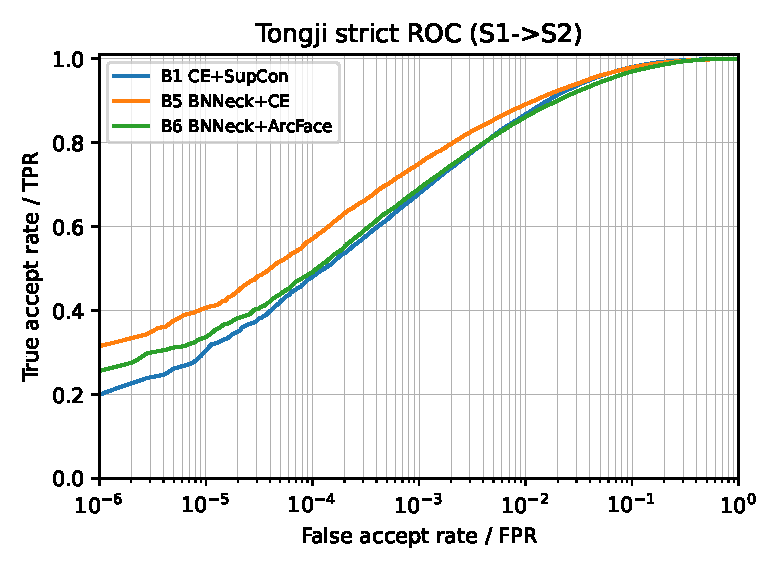
\includegraphics[width=0.48\textwidth]{figures/roc_tongji_b1_b5_b6_s1_to_s2.pdf}
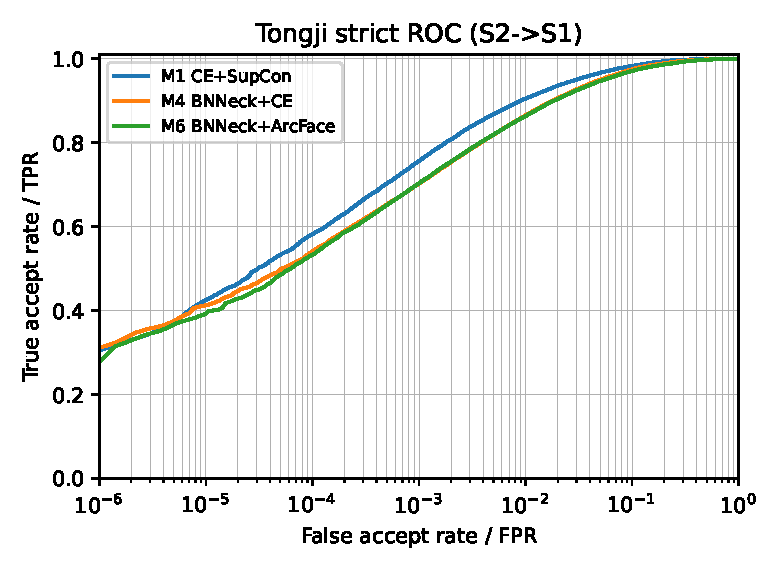
\includegraphics[width=0.48\textwidth]{figures/roc_tongji_b1_b5_b6_s2_to_s1.pdf}
\caption{Strict Tongji ROC curves for B1, B5, and B6, averaged over three seeds within each session direction. The curves emphasize low-FAR verification behavior under the palm-class-disjoint cross-session protocol.}
\label{fig:strict_tongji_roc_by_direction}
\end{figure*}

\begin{figure*}[t]
\centering
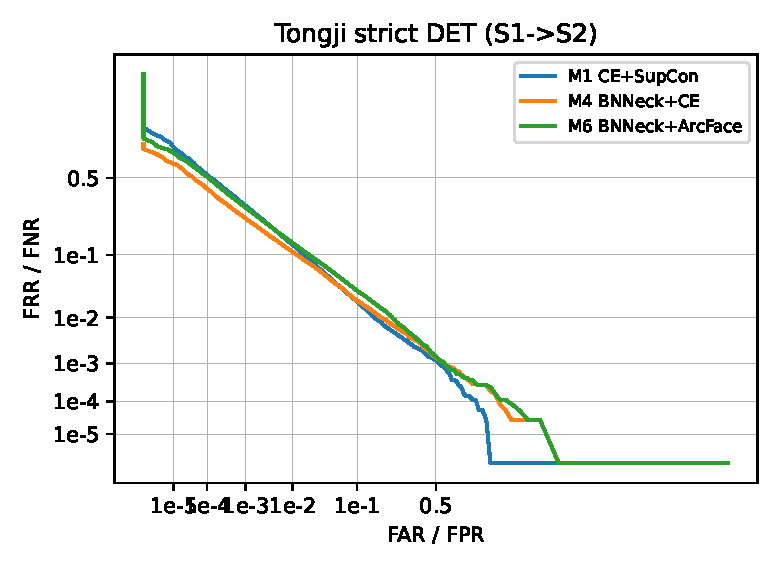
\includegraphics[width=0.48\textwidth]{figures/det_tongji_b1_b5_b6_s1_to_s2.pdf}
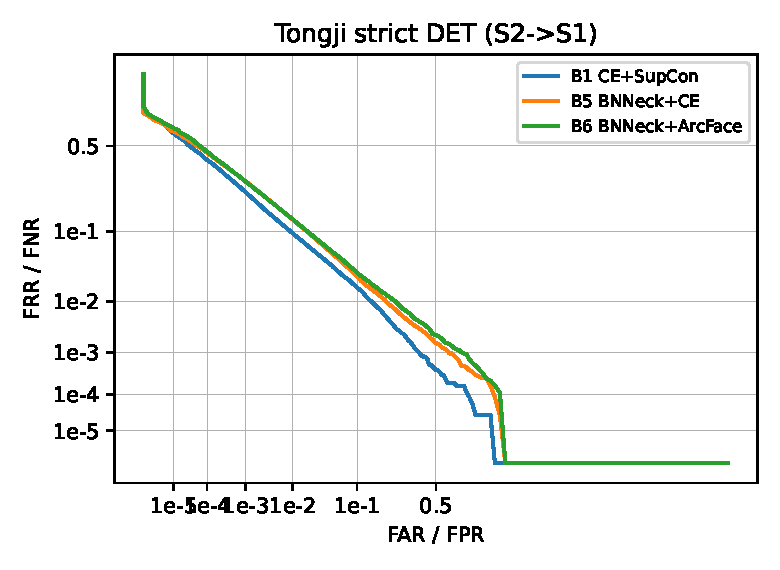
\includegraphics[width=0.48\textwidth]{figures/det_tongji_b1_b5_b6_s2_to_s1.pdf}
\caption{Strict Tongji DET curves for B1, B5, and B6. The DET view highlights that component behavior changes with session direction and that BNNeck+ArcFace does not provide a direction-invariant improvement.}
\label{fig:strict_tongji_det_by_direction}
\end{figure*}

\begin{figure*}[t]
\centering
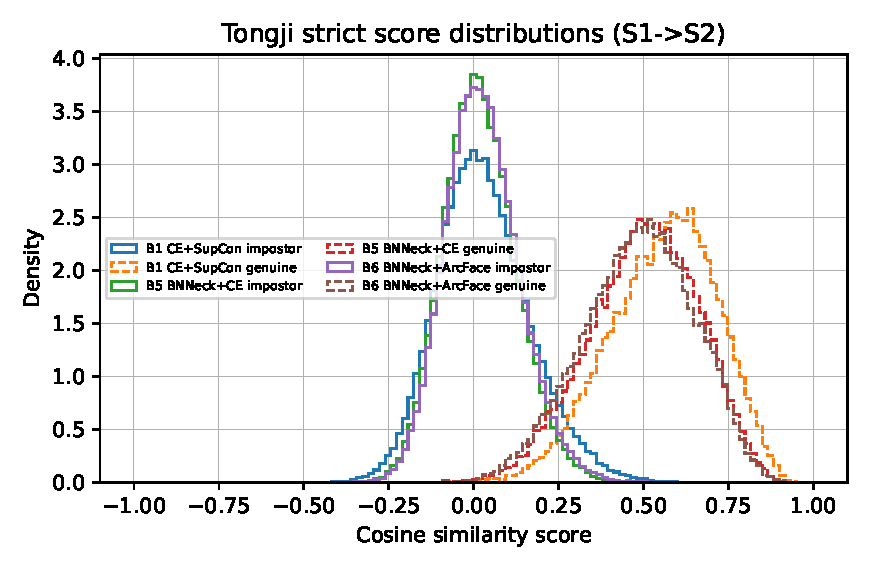
\includegraphics[width=0.48\textwidth]{figures/score_hist_tongji_b1_b5_b6_s1_to_s2.pdf}
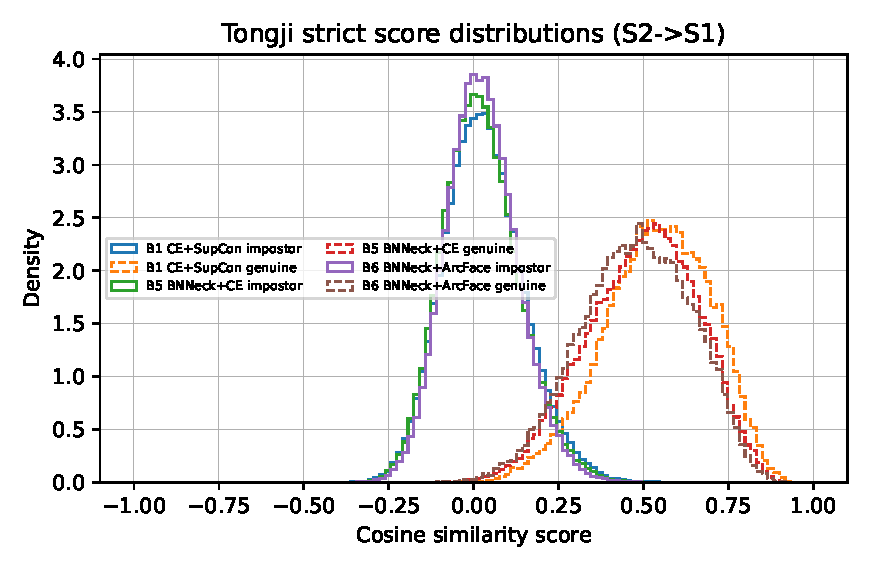
\includegraphics[width=0.48\textwidth]{figures/score_hist_tongji_b1_b5_b6_s2_to_s1.pdf}
\caption{Strict Tongji genuine and impostor score distributions for B1, B5, and B6. Dashed curves denote genuine-pair scores and solid curves denote impostor-pair scores. The distributions provide a score-level view of the direction-sensitive verification behavior.}
\label{fig:strict_tongji_score_hist_by_direction}
\end{figure*}
